\graphicspath{{05-EMR/Figures/}}

\section{Electron Muon Ranger}
\label{Sect:EMR}

\subsection{Introduction}
\label{SubSect:EMR_Intro}
 François provided this

The Electron-Muon Ranger (EMR) is a fully-active scintillator detector~\cite{2016JInst..11T10007}. It can be classified as a tracking-calorimeter as its granularity allows for track reconstruction. The EMR consists of extruded triangular scintillator bars arranged in planes. One plane contains 59 bars and covers an area of 1.27\,m$^2$. Each even bar is rotated by 180 degrees with respect to the odd one. A cross-section of bars and their arrangement in a plane is shown in Fig.~\ref{fig:EMR}. This configuration does not leave dead area in the detector for particles crossing a plane with angles that do not exceed 45 degrees with respect to the beam axis. Each plane is rotated through 90 degrees with respect to the previous one, such that a pair of planes defines a horizontal and vertical $(x, y)$ interaction coordinate. The light, produced when a particle crosses a bar, is collected by a wave-length shifting (WLS) fibre glued inside the bar. At both ends, the WLS fibre is coupled to clear fibres that transport the light to a photomultiplier tube (PMT). Signals produced in a plane are read out collectively on one end by a single-anode PMT for an integrated charge measurement and separately on the other by a multi-anode PMTs for individual bar hit reconstruction. The full detector is composed of 24 X--Y modules for a total active volume of $\sim 1$\,m$^3$.

\begin{figure}
	\begin{center}
		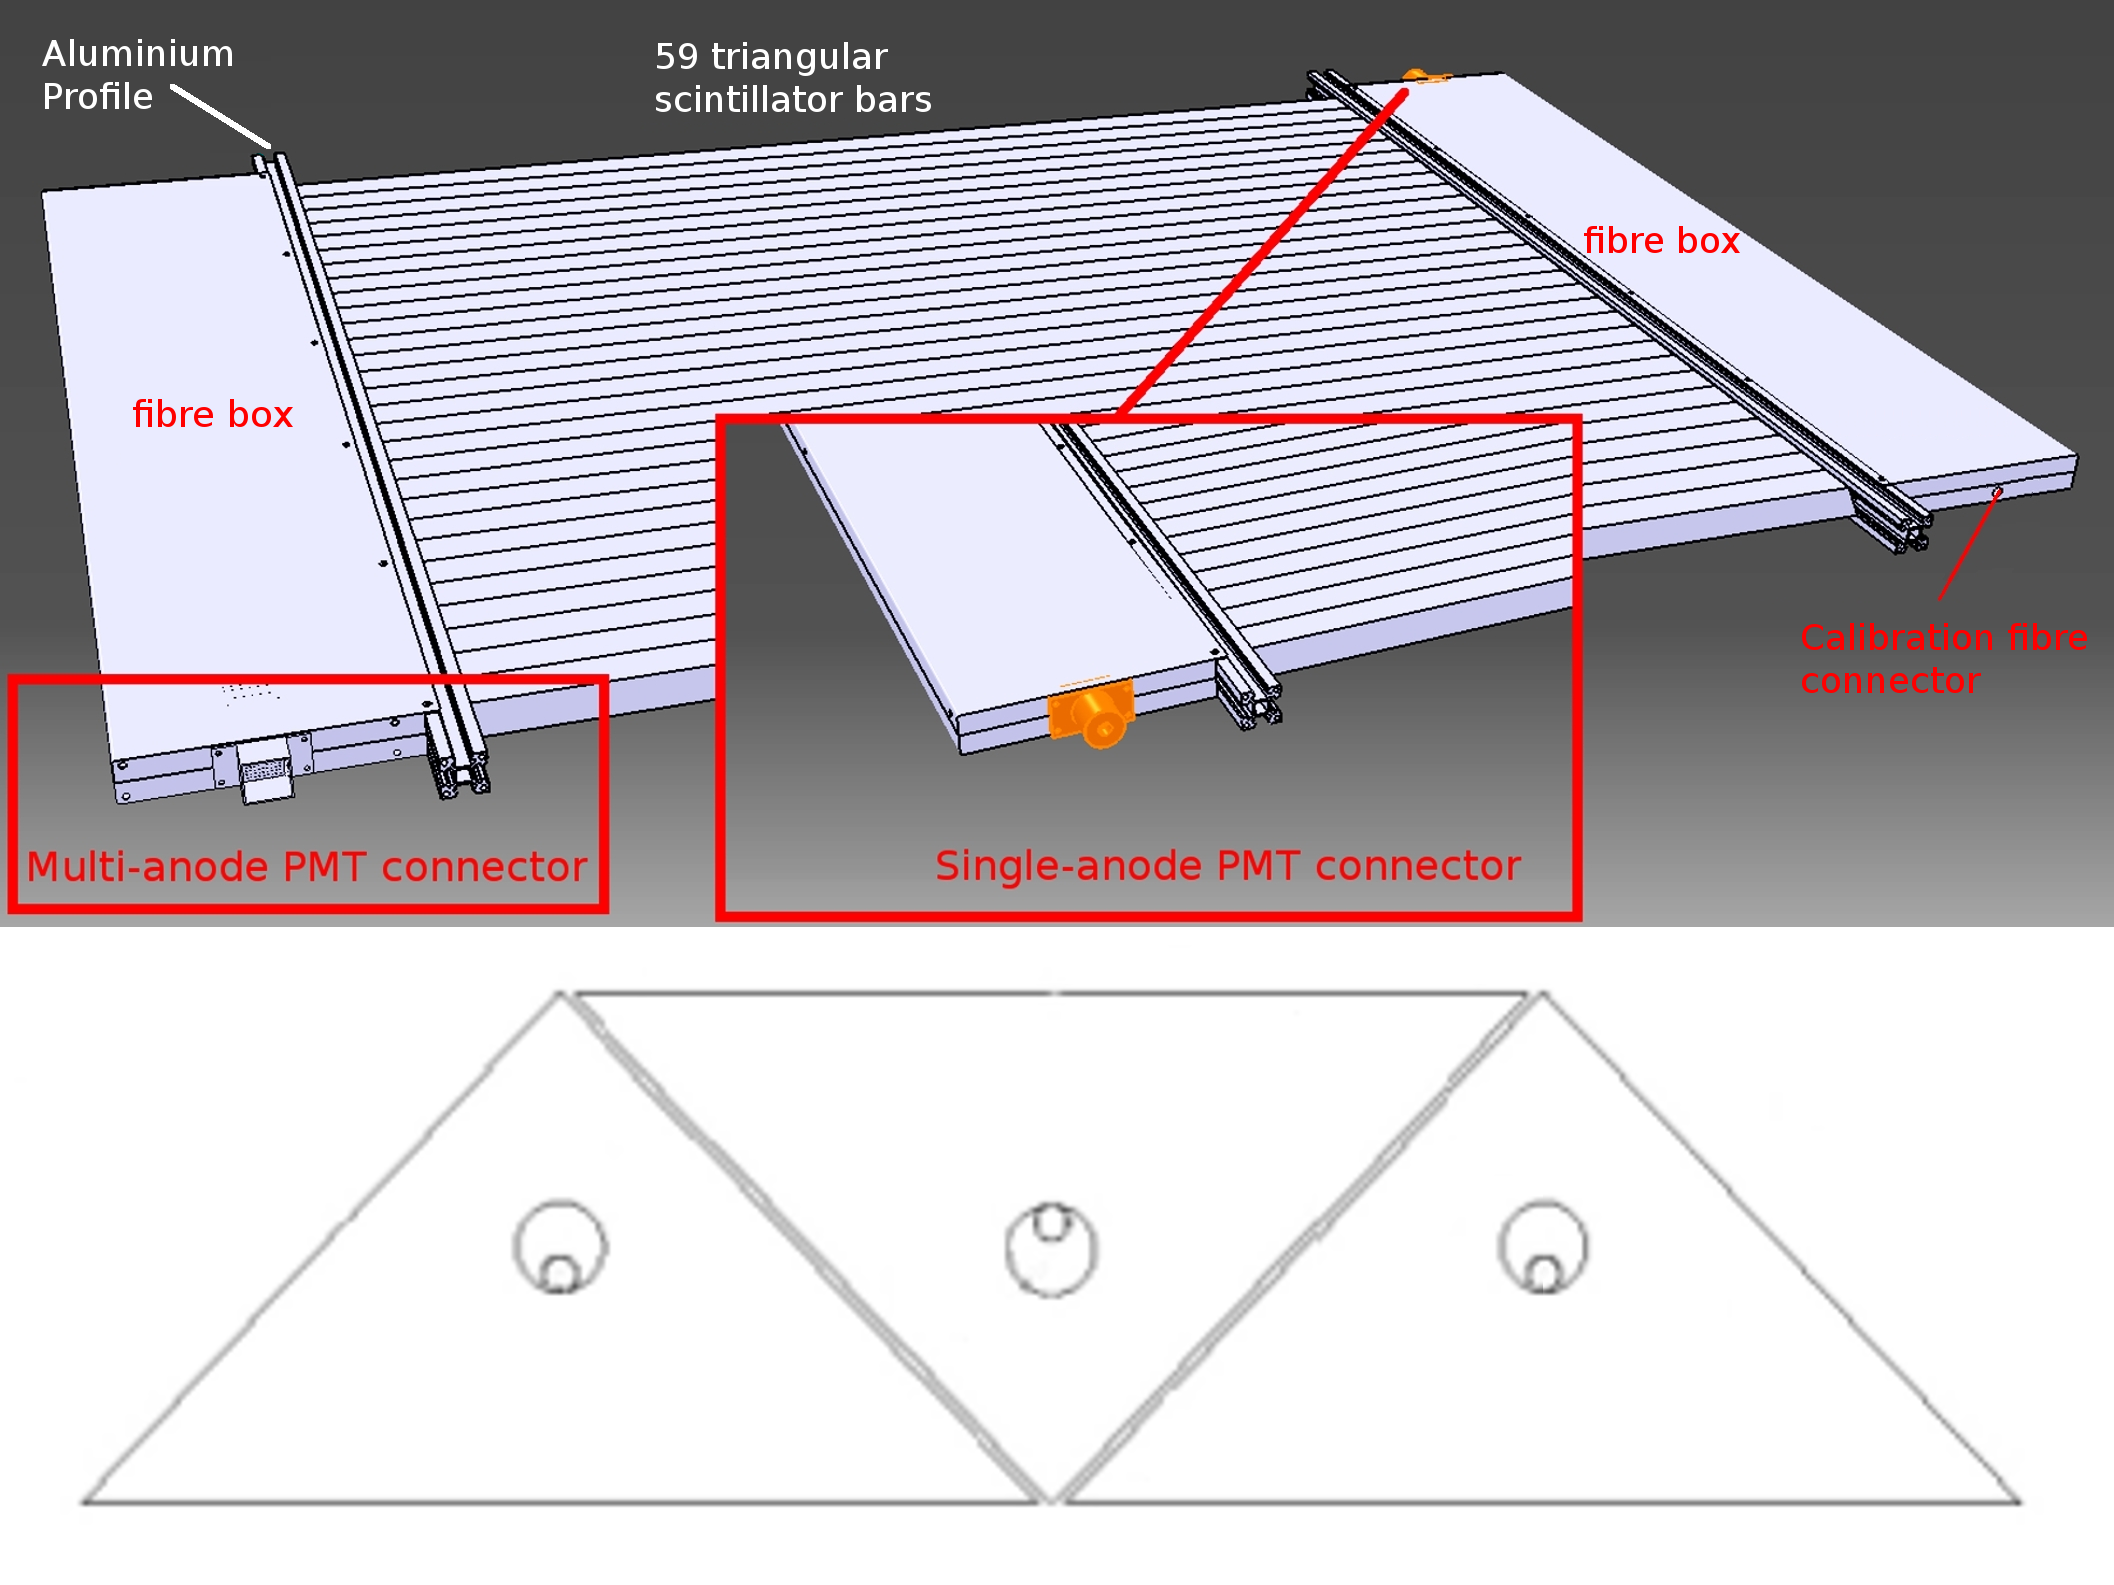
\includegraphics[width=0.465\columnwidth]{./05-EMR/Figures/EMR1.png}
		\hfill
		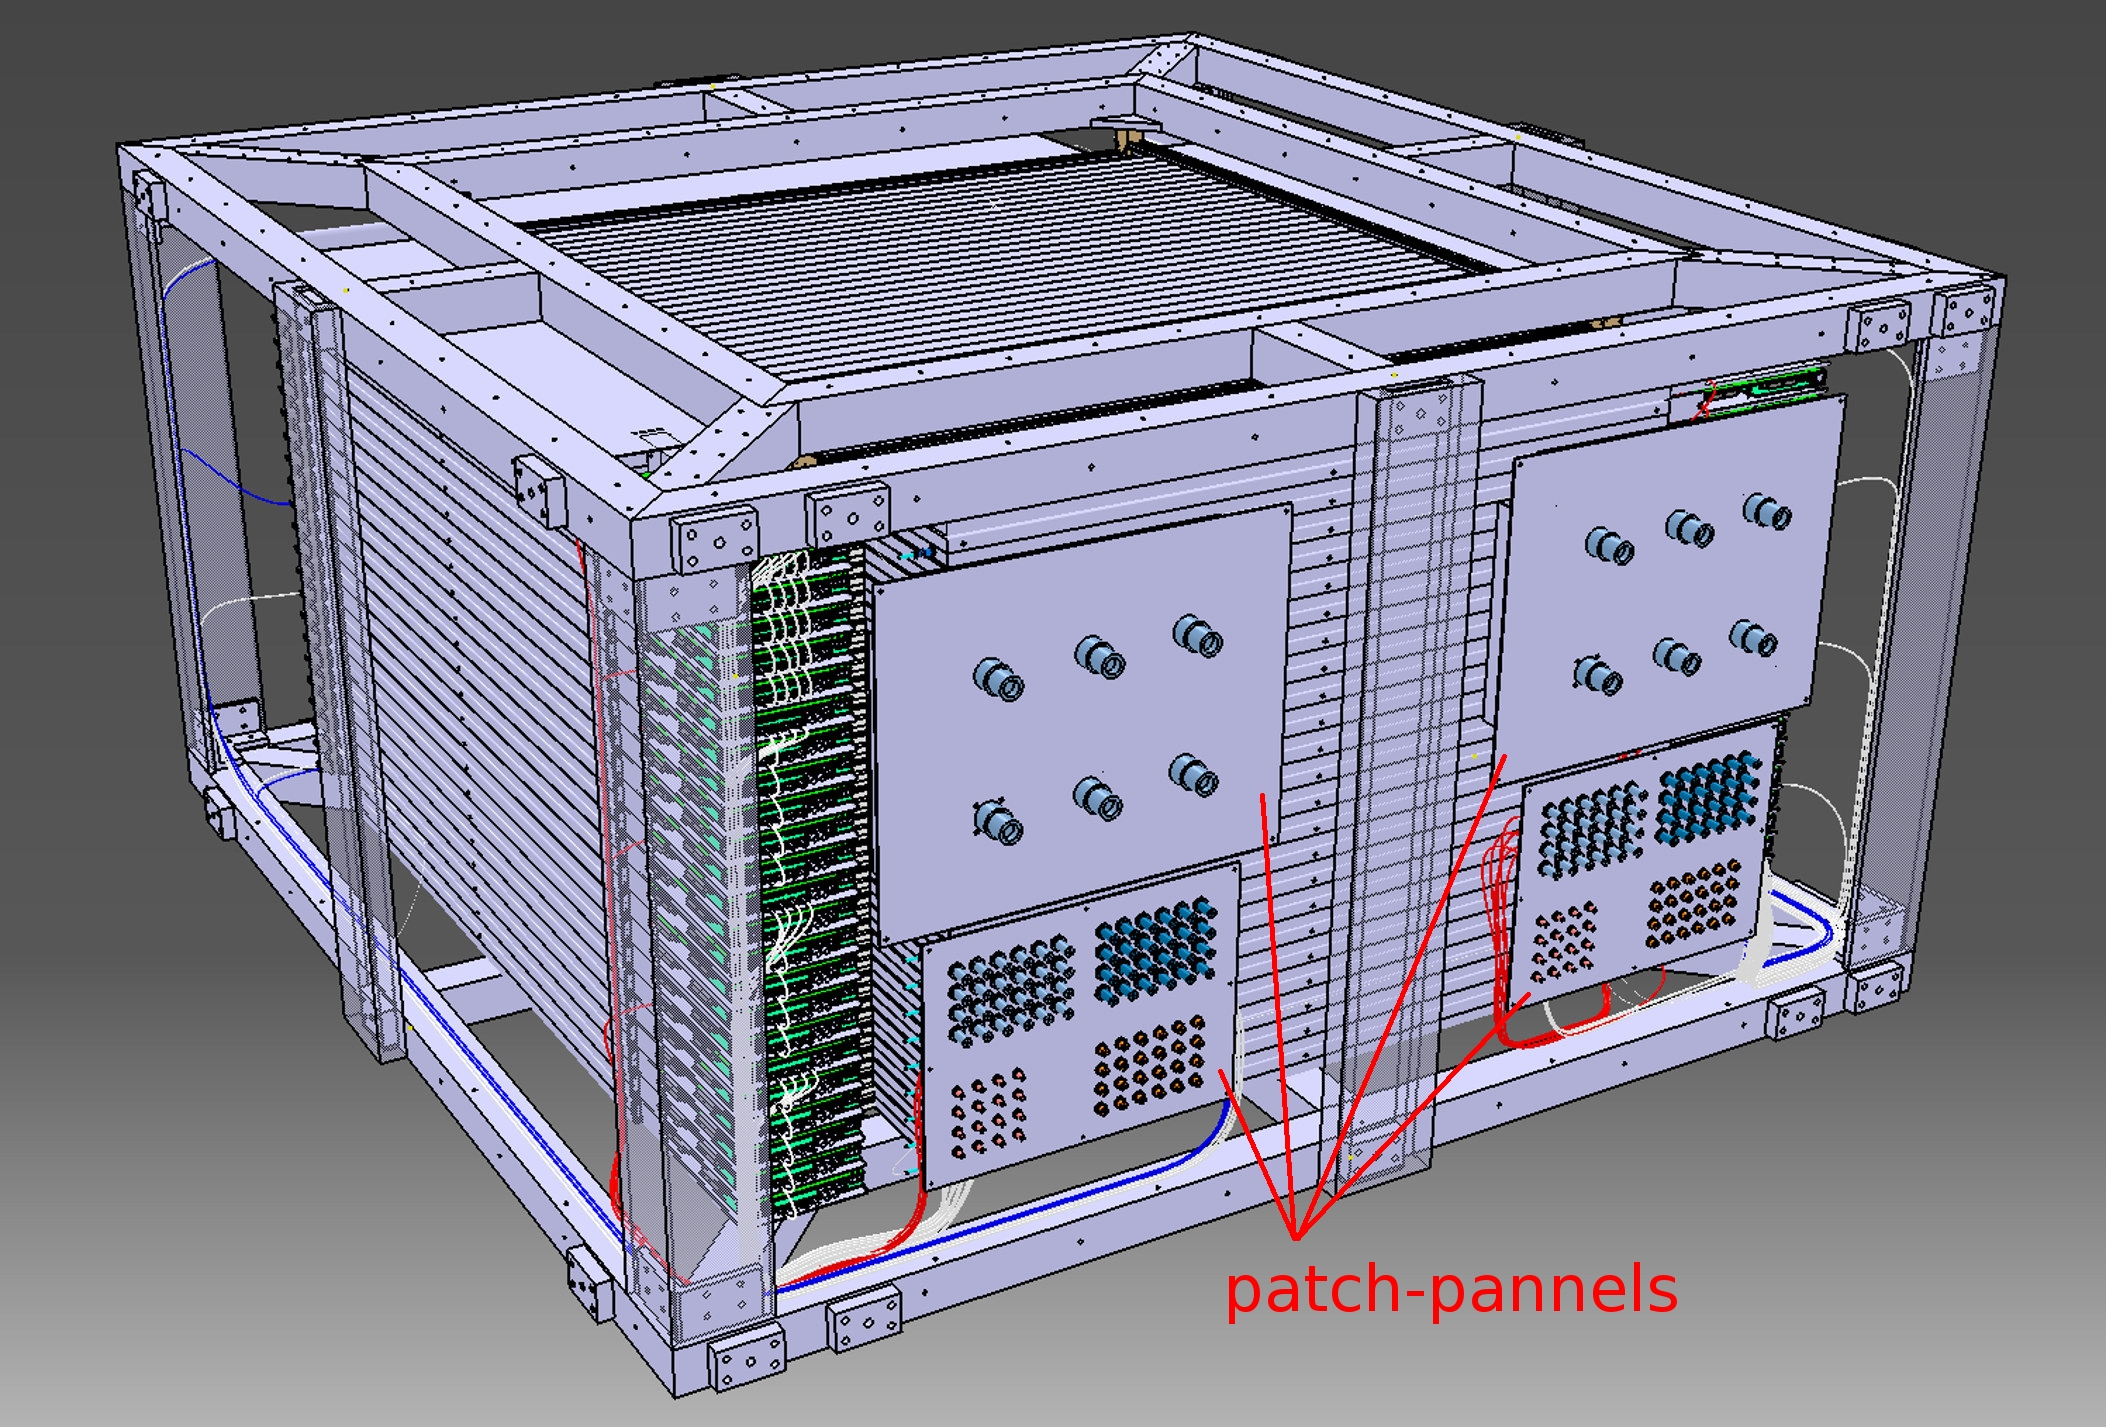
\includegraphics[width=0.515\columnwidth]{./05-EMR/Figures/EMR2.jpg}
		\caption{Drawing of one EMR plane (top left), cross section of 3 bars and their wavelength shifting fibres (bottom left) and drawing of the full detector (right).}
		\label{fig:EMR}
	\end{center}
\end{figure}

An array of analyses were conducted to characterize the hardware of the EMR and determine whether the detector performs to specifications~\cite{Drielsma:2017doj}. The clear fibres coming from the bars were shown to transmit the desired amount of light, and only four dead channels were identified in the electronics. Two channels had indubitably been mismatched during assembly and the DAQ channel map was subsequently corrected. The level of crosstalk is within acceptable values for the type of multi-anode photomultiplier used with an average of $0.20\pm0.03$\,\% probability of occurrence in adjacent channels and a mean amplitude equivalent to $4.5\pm0.1$\,\% of the primary signal intensity. The efficiency of the signal acquisition, defined as the probability of recording a signal in a plane when a particle goes through it in beam conditions, reached $99.73\pm0.02$\,\%.

The primary purpose of the EMR is to distinguish between muons and their decay products, identifying
muons that have crossed the entire cooling channel. Muons and electrons exhibit distinct behaviours in the detector. A muon follows a single straight track before either stopping or exiting the scintillating volume, while electrons shower in the lead of the KL and create a broad cascade of secondary particles. Two main geometric variables, the plane density and the shower spread, are used to differentiate them. The detector is capable of identifying electrons with an efficiency of 98.6\,\%, providing a purity for the MICE beam that exceeds 99.8\,\%. The EMR also proved to be a powerful tool for the reconstruction of muon momenta in the range 100--280\,MeV/$c$~\cite{2015JInst..10P2012A}.

\subsection{Performance}
\label{SubSect:EMR_Performance}
